\chapter{Text search}
\label{textsearch}
In order to create a modern, searchable e-mail interface, it is necessary to implement an algorithm that retrieves the wanted information quickly from a great amount of e-mails. The e-mail databases of some of the e-mail providers, such as Google or Outlook.com, have grown incredibly big throughout the years, containing billions of e-mails. Such databases are often far too big for naive approaches --- to find an email that contains specific keywords quickly (in milliseconds) we need a proper research of more advanced solutions for this problem.

This chapter describes the \emph{Text search}, its use in the search engines, its advantages and disadvantages comparing to the standard database search, its principles of use and implementation. 

Generally, the text search is used to find a document that contains a specific word structure in a database of text documents. In this chapter, we describe the overall process of \emph{indexing} the documents in such a database, and searching through them.

A \emph{document} is a single file of words, usually plain-text, processed and stored in the database: They are preprocessed before getting stored in order to simplify the search processing, for example by removing some unwanted (irrelevant for search) parts of the original text, such as various auxiliary words\footnote{Including e.g. articles, prepositions and conjunctions, these are usually called stop-words.} or markup, and split into so-called \emph{terms}. The terms are `clean' representations of the document content which are then stored in the database, together with the identification of the document they originated from. The list of split and processed terms associated to their documents is usually called a \emph{text-search index}. We describe this preprocessing, also usually called \emph{text analysis}, closer in \autoref{analysis}; indexing is described later in \autoref{index}.

The preprocessing of the document, as well as the searching itself, is usually done by a \emph{search engine}. A search engine is a system that integrates many text-search-related techniques to provide a coherent implementation of the indexing and querying functionality. In \autoref{engines}, we explain closer how the modern search engines work: The user requests sent to the search engine are called \emph{queries}. Each query lists some requested text words together with additional search criteria. The text in the query is processed by the same analysis that the documents are, to produce a simplified query of terms suitable for looking up in the database. The \emph{match} is the result of the search that is returned by the search engine as an answer to the given query. In other words, the match is a list of documents (in the most basic case it only contains document IDs) that
satisfy the criteria given by the query (e.g. contain the requested words).

Some search engines allow to structure the inner contents of the documents into \emph{fields}: Instead of treating all terms equivalently, users may separate them into the sets represented by the fields. A field is usually identified by string name, and contains a separately-searchable text value. For example, library databases may use fields such as \texttt{title}, \texttt{authors} or \texttt{topic}. This not only simplifies the user interface of the search, but also lowers the amount of data that need to be examined by the engine upon processing the query, because only the specific fields may be examined.

A simple diagram of the whole search cycle is provided in \autoref{fig:basic-chart}.
\begin{figure}
\centering
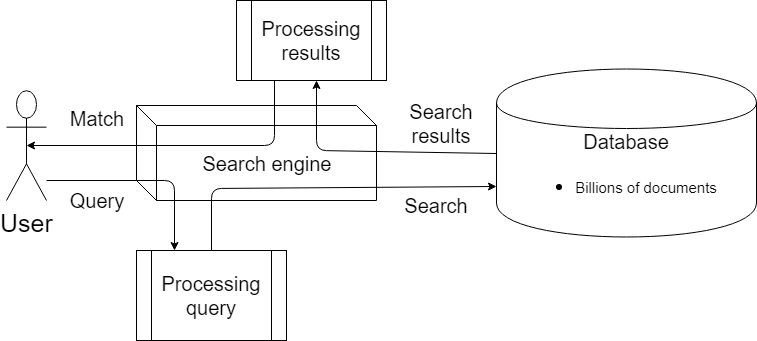
\includegraphics[width=\textwidth]{img/basic_chart.png}
\caption{A simplified view of the search cycle.}
\label{fig:basic-chart}
\end{figure}

In the following sections, we explain how the text search actually works, what processes are necessary for it to work efficiently and how to implement it.


\section{Text analysis}
\label{analysis}
There are many problems with word matching. Should  "ring" and  "Ring" match? Or  "swear" and  "swears"? In the natural human perception, we know that simply having the word at the beginning of the sentence (i.e. capitalized) does not change the meaning of the word. It is the same word as its non-capital version. We learned that "swear" and  "swears" are the same word, just in a different form. The search engine does not know that and we have to provide him with exact rules that he processes the words of the text as similarly to our perception as possible. This process is called \emph{text analysis}

Before we store the terms into the index, we need to preprocess them.
The text search analyzers are systems that process the words of the text and store them into the index. In reality, it is quite common that they treat the data in a natural way. Standard analyzers could remember the relative position, skip the insignificant words (such as "the"), treat certain fields as an exact type (e.g. date). Depending on the language, the analyzers can also decide to store the same word for its different word forms. For example, both words "forgot" and "forgotten" can be placed under the word "forget".

Generally, there are two phases of the text analysis, the \emph{tokenization} and the \emph{mapping}. \emph{Tokenization} is mandatory for creating the index but \emph{mapping} is optional and used only when needed.

The tokenization of the string is further subdivided into the following stages~\cite{elastic}.
\begin{enumerate}
\item First stage is the \emph{characters filter}. It is a preprocessing of the text before tokenization. It converts the text to the form that will be more simple to tokenize. For example, it is used to strip out HTML tags or convert \& to "add".
\item Then comes the tokenization itself. The string is split into the individual terms, accordingly to the defined analyzing parameters. The most simple tokenizers split the text whenever they encounter punctuation or whitespace, while removing the delimiter from the term.
\item The last stage is similar to the characters filter, the terms are post-processed by the \emph{tokens filter}. These filters change terms into their simplified forms, such as base forms, for easier future searching. The most common filters are lowercasing, removing the words with no possible significance to the search (stop words, e.g. "and", "the" etc.) or even adding words, such as synonyms.
\end{enumerate}

\subsection{Mapping}
As we mentioned before, there is more to the text analysis than the tokenization. We can tell the search engine how to treat specific fields and their values. For example, it is possible to have a field that contains only numbers. The search engine should understand that the value is not a simple plain string but a number. Later, it can make use of this type. For instance, the search engine can sort the results by this field. This technique is called mapping. 

Mapping is the process of defining how a document, and the fields it contains, are stored and indexed~\cite{elastic}. Which fields should be full-text fields, which should be numbers, booleans, date values, or not analyzed at all. Some search engines, for example ElasticSearch, offers the possibility to map a field using a specific language analyzer. If a field is supposed to contain only french words, the analyzer can understand the syntax of the French language and match it accordingly. For example, the word "anneau" ("ring" in English) and the word "Anneaux" have the same base form for the French language analyzer. The English language analyzer has a very little chance to understand that. Search engine remembers the specific settings for each field and processes the queries against them accordingly as well.

Different search engines use different approaches to the text analysis. How deeply is the text to be processed is mainly up to the developer that sets up the search engine.
For the purposes of this thesis, the most convenient way was to analyze almost every field. We wanted that the date of received/sent e-mail is treated as a date (milliseconds since certain date in the past) and that the results can be sorted by this value. On the other hand, there was no need to analyze fields such as \texttt{messageid} since in order to find a match, we are supposed to know the exact value. 
We did not specify any language analyzer as the users of KamehaMail can be of different nationalities, consequently writing their e-mails in different languages.

We used tokenization and mapping to process the text into terms and now we want to store them.
\section{Indexing and inverted indexes}
\label{index}
Much research has been performed to design efficient
index structures for database and information retrieval
systems~\cite{structs}. There was a need to find an ideal data structure to store and retrieve data from a database full of plain-text documents as quickly as possible. In order to do reach the solution, some sort of indexing of the split terms was needed.
A standard forward index appeared to be inefficient for the full-text search. The goal is not to look for the documents but for the words in them. Thus, the most efficient index structure is an \emph{inverted index}~\cite{invertedfiles}.

An \emph{inverted index} is structured the opposite way to the forward index. Instead of having a list of documents along with lists of terms accordingly, inverted index contains a list of terms and for each the documents that contain them. The difference between them is shown in the \autoref{table:forward-inverted}.

\begin{table}[t]
\centering
\renewcommand{\arraystretch}{1.4}
\begin{tabular}{c l}
\toprule
Inverted Index\\
\midrule
Term 1 & List of documents \\
Term 2 & List of documents \\
Term 3 & List of documents \\
Term 4 & List of documents \\
\dots & \dots \\
\bottomrule
\end{tabular}
\qquad
\begin{tabular}{c l}
\toprule
Forward Index\\
\midrule
Document 1 & List of terms \\
Document 2 & List of terms \\
Document 3 & List of terms \\
Document 4 & List of terms \\
\dots & \dots \\
\bottomrule
\end{tabular}
\caption{An inverted index (left) and a forward index (right).} 
\label{table:forward-inverted}
\end{table}

There exist two major types of inverted indexes. An \emph{inverted file} (or \emph{document-level index}) and a \emph{full inverted index} (or \emph{term-level index}). The difference is that inverted file is used only for accessing the documents of the corresponding term. It is sufficient when no other information than document's ID is needed. A full inverted index has complete information about the term in the file (e.g. position) which makes it far bigger and harder to maintain, however indispensable in certain use cases, for example, when the word position is needed.

An inverted index consists of two main parts.
\begin{enumerate}
\item The first part is the \emph{vocabulary}. It is a list of all distinct terms of all documents. Each of them can contain information about document count and about their \emph{inverted lists}. The inverted lists are associated to their respective terms directly, as a list or by a pointer to the corresponding part. The position of a word is stored as well, if it is not the document-level index. This list is ordered.
\item The second part is an \emph{inverted list} which is a list of all documents where the word appeared. These lists can be represented as pairs \((d, f_{d,t})\) where \(d\) represents the identifier of the document and  \(f_{d,t}\) is the associated set of frequencies of the term \(t\) in the document \(d\)~\cite{invertedfiles}.
This list is ordered as well.
\end{enumerate}

A simple database of documents is provided in the \autoref{table:data-ex} for the presentation purposes. Each document in the table is uniquely identified by its \texttt{ID} field. The actual text of the quote is stored in the \texttt{Text} field. The \texttt{Author} field contains the author of the quote. As we mentioned before, the terms are processed and stored to the index structure which is shown in \autoref{table:invlist-ex}. Notice that the inverted index provided in the example is made only of the field \texttt{Text}.

\begin{table}[t]
\centering
\renewcommand{\arraystretch}{1.4}
\begin{tabular}{c p{20em} l}
\toprule
ID & Text & Author\\
\midrule
1 & Your time will come. You will face the same Evil, and you will defeat it. & Arwen \\
2 & The Ring has awoken, it has heard its masters call. & Gandalf \\
3 & We swears, to serve the master of the Precious. We will swear on\dots on the Precious! & Gollum \\
4 & You shall not pass! & Gandalf \\
\bottomrule
\end{tabular}
\caption{A simple database of quotes from Lord of the Rings.} 
\label{table:data-ex}
\end{table}

\begin{table}[t]
\renewcommand{\arraystretch}{1.4}
\resizebox{\textwidth}{!}{
 \begin{tabular}{c c} 
 \toprule
 term \(t\) & \((d, f_{d,t})\) \\ 
 \midrule
 and & (1, 1) \\
 awoken & (2, 1) \\
 call & (2, 1) \\
 come & (1, 1) \\
 defeat & (1, 1) \\
 evil & (1, 1) \\
 face & (2, 1) \\
 has & (2, 2) \\
 heard & (2, 1) \\
 it & (1, 1),  (2, 1) \\
 its & (2, 1) \\
\bottomrule
\end{tabular}
\quad
 \begin{tabular}{c c} 
 \toprule
 term \(t\) & \((d, f_{d,t})\) \\ 
 \midrule
 master & (3, 1) \\
 masters & (2, 1) \\
 not & (4, 1) \\
 of & (3, 1) \\
 on & (3, 2) \\ 
 pass & (4, 1) \\
 precious & (3, 2) \\
 ring & (2, 1) \\
 same & (1, 1) \\
 serve & (3, 1) \\
 shall & (4, 1) \\
\bottomrule
\end{tabular}
\quad
 \begin{tabular}{c c} 
 \toprule
 term \(t\) & \((d, f_{d,t})\) \\ 
 \midrule
 swear & (3, 1) \\
 swears & (3, 1) \\
 the & (1, 1),  (2, 1),  (3, 3) \\
 time & (1, 1) \\
 to & (3, 1) \\
 we & (3, 2) \\
 will & (1, 3),  (3, 1) \\
 you & (1, 2), (4, 1) \\
 your & (1, 1) \\
 & \\
 & \\
\bottomrule
\end{tabular}
}
\caption{A document-level inverted index for the database shown in the \autoref{table:data-ex} with only word occurrences.}
\label{table:invlist-ex}
\end{table}

Nowadays, there are plenty of variations for the inverted index structure. Several possibilities were mentioned in the article written by Mahapatra and Biswas~\cite{invindex}. For instance, some of them store meta data. Apart from the additional information stored for each word (such as the frequency of the occurrence or the word position), these implementations contain meta-information about each hit. \emph{Hit} is an exact word position in the document. These meta data may contain information such as font type, font size, text type etc\dots Other solutions mentioned in the article implement both types of the inverted indexes, the full inverted index and the inverted file, each for different situations.

Creating an inverted index is a simple task. However, it can be challenging to create it without wasting memory and CPU. Advancements in the hardware do not provide any significant help because the collections are growing in size even faster. An efficient way is needed for creating, storing and maintaining the index.

\subsection{Construction of inverted index}
The fastest and the most simple way to construct an inverted index is to build the whole collection in memory. However, this approach is not possible for bigger collection (i.e. billions of documents, terabytes of data). Such collections do not fit in the memory and disk has to be used which is always costly. An optimized method that
creates small, memory fittable inverted lists, stores them to disk and merges them when all is done is needed. Moffat and Bell or Heinz and Zobel described several methods solving this problem~\cite{invindex}.

\subsection{Structure of the inverted index}
The article written in 1996~\cite{structs} defines two following approaches for the inverted index structures.

The first approach is to maintain an inverted index only for the document access. Specifically, only document IDs are returned upon a matching query. A postprocessing is needed to retrieve additional information about the document, if wanted. That is done by using a term-level index. This approach has a significant disadvantage, as the number of the matching documents can be large, the postprocessing can be time consuming. Although, it can be improved by using an internal tree representation.

The second approach is about having an index for each element type. It may create a huge space overhead as each term must appear in every index. There were attempts for removing the duplicates, for example by using a combined vocabulary. Nevertheless, the space overhead was still far too great.
Many different possible structures exist which take care of the duplicates and improve the consequential space overhead.

To further reduce space consumption, compressions can be applied on the inverted lists~\cite{invindex}. For example, instead of storing all the numbers as 32-bit integers, variable-length numbers can be used.

\subsection{Segmentation}
The maintenance of already existing inverted index also causes an issue. Inserting a new element into a sorted list and updating the whole index with possibly billions of documents directly is too expensive.

ElasticSearch uses the principles of \emph{segmentation} as defined by Lucene and the following facts will be interpreted as explained in the guide for ElasticSearch~\cite{elastic}. 

Instead of rewriting the whole inverted index again upon each new entry, completely new indexes are created with the recent results. Such supplementary index is called a \emph{segment}. Lucene describes the index as a collection of segments and a commit point. Commit point serves as a common entry point for its segments, the query is performed against it, the commit point then distributes the query to all its segments and returns the results combined.
The \autoref{fig:commit} shows an example of the segmentation.
\begin{figure}
\centering
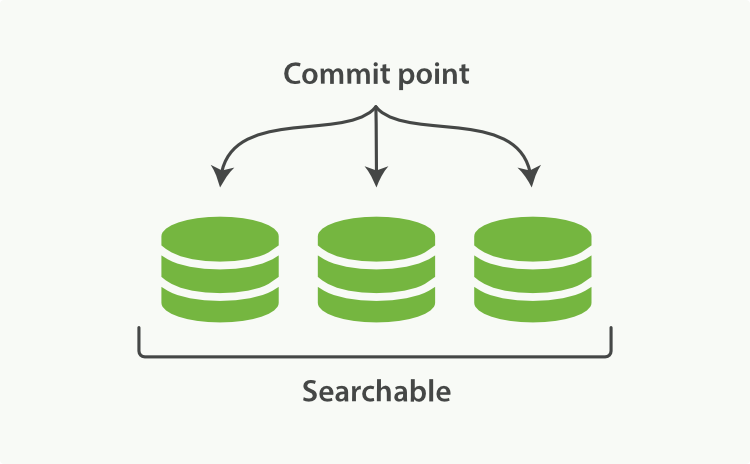
\includegraphics[width=.8\textwidth]{img/commit.png}
\caption{A commit point for three segments of the index.}
\label{fig:commit}
\end{figure}
This may cause an issue because the approach may create an enormous amount of small segments which consume additional CPU and memory, rendering inverted indexes inefficient.
It can be at least partially improved by merging the segments, transparently for the incoming search query and the user. It is most convenient to run this process when a new, not yet committed (not yet written to the specific commit point) segment has been set. Currently committed segments are taken along with the new uncommitted one and merged. The new merged segment is then committed into the commit point and the old ones are to be removed. To remove them safely, the search engine must be sure that there are no searches being performed on them which usually delays their removal.

The problems mentioned above are not the only problems concerning inverted indexes. However, they are efficiently solved by the search engine we integrated to the application, ElasticSearch. The specifications of ElasticSearch are mentioned in \autoref{es}. 

\section{Query structure}
\label{query}
Once the database is constructed and prepared for the text search queries, it is possible to search in it. Search engines usually provide an API to make the communication with them (i.e. send the queries and receive the match data) possible. The following examples are written in a JSON-based syntax, similar to the ElasticSearch~\cite{elastic} but simplified for presentation purposes. The queries are effectively performed against the inverted index to the database shown in \autoref{table:data-ex}. The \texttt{Text} field part of the database is displayed in \autoref{table:invlist-ex}.

A simple query looking for the term "ring" is shown in the following example:
\begin{code}
{ "query": { 
    "term" : "ring"
} }
\end{code}
The second document contains term "ring" and it is the only match. The most basic result to the above query returns only the matched documents' IDs:
\begin{code}
{ "hits": [
    { "ID" : 2 } ] 
}
\end{code}
\texttt{Hits} is an array of results. For each matching document, it contains at least the document's ID. Nonetheless, there are cases where we want to have more information about the document than its ID. For example, other contents of the matching documents or the relevancy of the document to the given query.

Queries can be more complex, defining different logical search criteria. We can use logical NOT (for the unwanted terms), AND (for multiple terms) and OR (for optional matches). In the following example, user is looking for those documents that contain terms "master" and "precious", cannot contain term "ring" and optionally may contain term "evil":
\newpage
\begin{code}
{ "query" : { 
     "bool" : {
       "must" : {
        "term" : "precious",
        "term" : "master"
      },  "must_not" : {
        "term" : "ring"
      },  "should" : {
        "term" : "evil"
      }
} } }
\end{code}
The first document contains the term "evil" but it does not have any of the obligatory terms, so it will not be a match. The document 4 does not contain any of obligatory terms. The document 2 neither and furthermore it contains the forbidden term "ring". The document 3 contains both of the obligatory terms, does not contain term  "ring" which makes it the only match. It is still a match even if it does not have the term "evil" which was meant to be optional.

In the previous examples, the search field was not specified so the search engine looked at all fields. If we want to find all of the Gandal's quotes, we can write the following query:
\begin{code}
{ "query": { 
    "term" : "gandalf"
} }
\end{code}
This is a legit query that returns documents 2 and 4 as results. But it searches through all the fields, \texttt{Text} and \texttt{Author}. This may be time consuming. Depending on the length of the Gandalf's quotes and the amount of his quotes in the database, such queries can be inefficient. 
To save time, we specify the field in the following example:
\begin{code}
{ "query": { 
    "term" : {
        "Author" : "gandalf"
} } }
\end{code}
Let's say that this time we want that the search engine returns more information about the matching document, for example the text of the quote:
 \begin{code}
{ "hits": [ { 
      "ID" : 2,
      "_source" : {
        "Text"  : "the ring has awoken it has heard its
                        masters call" 
      } }, { 
      "ID" : 4,
      "_source" : {
        "Text"  : "you shall not pass" 
} } ] }
\end{code}

\paragraph{Search details description.}
The full-text search does not look for a simple key but rather for content~\cite{invertedfiles}. When the user provides a query, he is looking for the meaning inside the text according to it. The search engine should evaluate the query not only in a lexical way but also in a contextual way. In order to ensure this behaviour, the search engine needs exact rules for ranking the results appropriately. First of all, it uses the very same analyzer for the query as it used for the documents stored in the database.
This method ensures that upon looking at a specific word, we will get its other word forms as well. In certain implementations even synonyms.

Typical steps for the query evaluation are the following~\cite{elastic}. 
\begin{enumerate}
\item First, the type of the field in the query is checked, to determine if it should be analyzed or not.
\item If necessary, the query string is analyzed using the according analyzer.
\item Then, the search engine looks into the inverted index and finds the IDs of the matching documents.
\item Using the matching document IDs, the search engine can provide, if requested, various additional information, such as relevance of the match or values of other fields of the matching documents.
\end{enumerate}

In case that query fails and does not find any matching documents or the match does not evaluate as expected, the user can decide to refine the query in various ways. We already mentioned that the full-text search tries to find the most relevant results and sort them that way. The following sections details the ranking of the match.

\subsection{Relevance and effectiveness}
There is an issue of the quantification of the relevance. Is it possible to measure the relevance of a term in the document?
Relevance of word to the text can be considered subjective or inexact. The document can be relevant to the given query even though it contains none of the terms~\cite{invertedfiles}.

Because of this inexact attribute of the relevance, the attribute \emph{effectiveness}~\cite{invertedfiles} is preferred. The engine is considered to be effective if the number of the matched results is as close as possible to the expected results.
Effectiveness is typically described by two aspects, \emph{precision} and \emph{recall}. Recall measures the quality of the results, it is a fraction between the matches found and all the relevant matches. Precision measures the quantity of the results, it is a fraction between the relevant matches found and all matches found.
 
We want to know how to measure the relevance. The number indicating the relevance of a document to the given query is called the \emph{score}. In the following example, the score will be a number between zero and one. One means the result is as relevant as possible. Zero means the result is completely irrelevant and will not be displayed at all.
There are multiple ways to evaluate the score of the match~\cite{elastic}: the occurrences of the query in the document or the format of the term. Recall that some implementations of the inverted indexes contain meta data of the original text. In that case, it is simple to check if the querying term was a header or bold before the text analysis. Another method is to compute how big portion of the text the term takes. The following example searches for word "you" in \autoref{table:invlist-ex} and sorts the matches by the relevance of the term "you" in the matched documents:

 \begin{code}
{ "hits": [ { 
      "_id" : 1,
      "_score" : 36.5
    },
    { 
      "_id" : 4,
      "_score" : 23.5
} ] }
\end{code}

Two documents matched. For presentation purposes, we create a simple version of pseudo-procedure for evaluating the score of the match:
\begin{enumerate}
\item For each exact occurrence of the term, add 10 points to the score. Add 3 extra points for each capital letter in the occurrence.
\item For each similar occurrence of the term, add 5 points to the score (can be adjusted depending how similar the occurrence is). Add 1 extra point for each capital letter in the occurrence.
\item Add 0.5 point for each percent of the text the occurrence takes. If the occurrence takes generally 30\% of the text, add 15 points. (This can be normalized to the whole length of the text. The bigger the text, the less likely the term will be relevant).
\end{enumerate}
According to this algorithm, the document 1 has 2 * 10 points for the exact occurrences and 3 extra points for the capital letter, 5 points for a similar occurrence ("your") and 1 extra point because it starts with the capital letter again. Finally, "you" takes together almost 15\% of the whole quote, which means another 7.5 points are added, resulting in 36.5 points together for document 1.

The document 4 gets only 10 points for one occurrence and 3 points because it has a capital letter. The term takes roughly 21\% of the quote which means another 10.5 points are added, resulting in 23.5 points together for document 4.

This simple algorithm determined that term "you" is more relevant in the quote "Your time will come. You will face the same Evil, and you will defeat it" than in the quote "You shall not pass!".

The real implementation of the scoring algorithms can be far more complex, taking in consideration the length of the field or the inverse document frequency~\cite{elastic}. The ElasticSearch uses own formula which is mentioned \autoref{es}.

\subsection{Phrase query}
The user does not only searches for one term. The vast majority of the web search queries contain phrases, multiple words in a single query field. For the database search, it is an easy task to perform a phrase query --- if the document contains the phrase as it is, match it. The text search takes in consideration the relevance and it needs a way to measure the relevance of the phrase query as well. The user expects that the most relevant results should be those documents that contain the phrase as a whole. The more words in the phrase query are separated from each other in the document, the less relevant it should be. 

Three possible procedures were mentioned in the article written by Zobel and Moffat~\cite{invertedfiles}.

The first procedure is that the phrase is indexed as a term and that it has its own inverted list. This solution is often too space consuming, as it is impossible to predict which two-word pair phrases are necessary to be stored. Creating all possible two-word pairs creates an absurdly big collection (three-word, four-word\dots). It can be improved by partial indexing and combinations.

Another way is to simply split the phrase and run a separate query for each split term. This may possibly return seemingly irrelevant matches, as the words can happen to be anywhere in the document, have no actual meaning together and still be a well-ranked match.

Last mentioned procedure is to keep the word positions in the index so that the position of the phrase can be determined during evaluation.

These three procedures can cooperate together and the final implementation of the phrase query evaluation is possibly a combination of them. However pure use of only one of them will not return reasonable results.

The users of KamehaMail will very likely use phrase querying which is again handled by ElasticSearch.

We described all necessary things to understand the steps needed for a working search engine. In the following part, we look at the search engines themselves, compare them to the standard database search and provide some statistics about them.

\section{Search engines}
\label{engines}

\subsection{Comparison with relational indexing methods}
Search engines are similar to the database systems~\cite{invertedfiles}. The documents are indexed and stored in the database, the search engine evaluates the queries against the index and finds the match. However, there are differences mostly in the way the queries are performed and the way the documents are stored. For instance, the majority of the queries for the search engines are just lists of terms while the database systems are facing complex queries (SQL). On the other hand, the database systems are matching only specific logical condition, the search engines take in consideration the relevance of the document to the given query. Consequently, the database search returns all matches while the search engines return fixed number of matches, sorted by the score of relevance. Returning all matches would not be possible in certain cases because the result of the query may be huge (millions of documents).
That is because the resulting documents may contain terms that are at least in some minimal way similar to the query but almost completely irrelevant for the user.

\subsubsection{Advantages}
The main advantage of the text search comparing to the standard database search is in the way they process the words of the text.

Standard database search with its binary query cannot even partially understand the context of the text. It cannot make use of the index when looking for similarity. For example, if we want to find all Gandalf's quotes with possible suffixes (\texttt{WHERE Author LIKE Gandalf\%}), the standard database se\-arch does not use the index, it has to look at every row and check if it is a match. In many cases, that is an unwanted and insufficient behaviour. This also makes the standard database search slower, as it is not optimized for similarity searching.

We already know that text search understands the value of the data, refers to it as it was written in human language and behaves that way~\cite{elastic}. Many of the search engines are capable of matching synonyms or understanding the context. When we are looking for the phrase "Fox News", we actually do not want news about foxes but some news published by Fox News. Many distinct approaches of data evaluation can be defined to the specific fields by the developer. 

\subsubsection{Disadvantages}
There are few disadvantages to the text searching when comparing with the standard database search.

An index for a text search can be massively bigger than a standard B-Tree index. B-Tree is a self-balancing tree structure for searching, inserting and deleting in logarithmic time. A full text search index (or inverted index) contains duplicates, which can potentially make it several times bigger.

Another disadvantage is hard maintainability of the inverted indexes. The fact that the lists of documents are sorted and potentially large makes it difficult to insert into them in a reasonable time. However, there exist improvements as well.
 
\subsection{Web search engines}
Text searches most essential use is in the web search engines. They index the webpages and so provide an easier access to information that was inconceivable a few decades ago~\cite{invertedfiles}. Several of the following facts were published in the article written by Lawrence Page and Sergey Brin~\cite{google}.
They stated that developing a Web Search engine is a difficult task, as it has to process tons of web pages along with tons of search queries. The Web is rapidly growing every day, with more and more webpages being created. In the 1994, one of the first web search engines, the World Wide Web Worm had an index of 110,000 web pages. In the end of 1997, WebCrawler claimed to have from 2 million to 100 million documents. In the present, the biggest and the top search engine is Google. On the 12th of January, it stated that it had more than 47 billions of webpages indexed~\cite{wwwstats}, as we can see in \autoref{fig:graph_googleweb}. 
\begin{figure}
\centering
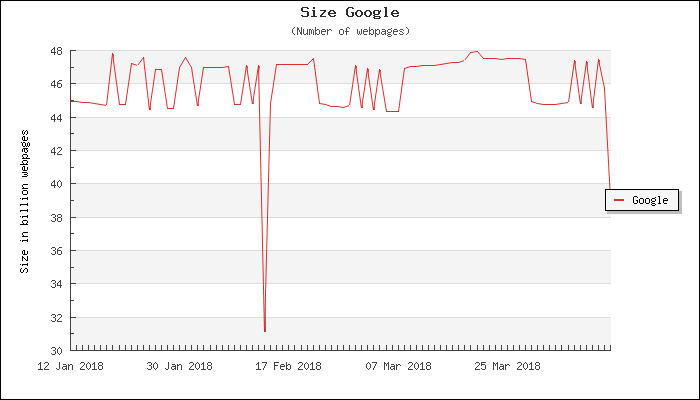
\includegraphics[width=.8\textwidth]{img/google_webpages.png}
\caption{The amount of webpages indexed by Google}
\label{fig:graph_googleweb}
\end{figure}
Google proved to be the most used web search engine by processesing the vast majority of all the web search queries. It held 81.53\% of the search engines market share from January 2017 to January 2018, as shown in \autoref{fig:graph_market}\footnote{provided by \texttt{netmarket.com}}.
\begin{figure}
\centering
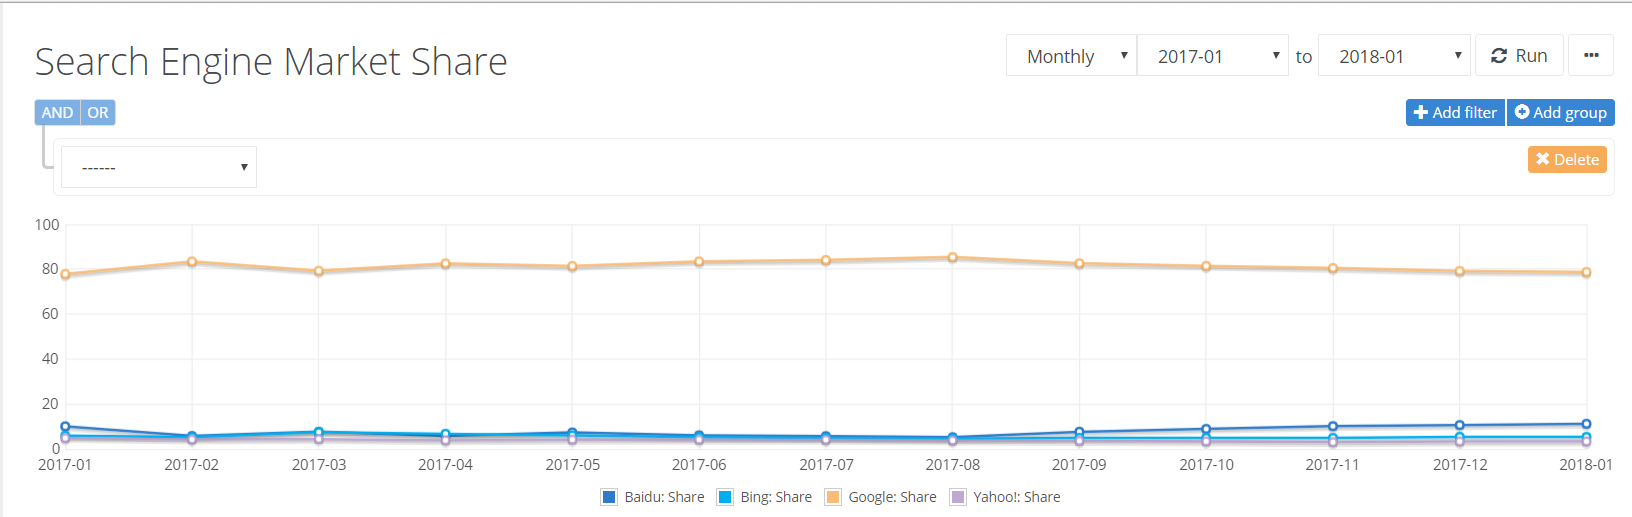
\includegraphics[width=.8\textwidth]{img/search_engine_market.png}
\caption{The search engine market on all platforms in 2017.}
\label{fig:graph_market}
\end{figure}

Complementary to the already mentioned automated search engines relying on keyword matching, there exist human maintained search engines. They may return more sufficient answers but are expensive to build and hard to maintain~\cite{google}.

The collections used by the search engines can be vastly distinct from each other: For example, they can vary in size. Some collections can be as small as tens of megabytes and grow each day by only few hundreds of documents. Others may contain tens of gigabytes (e.g. libraries) but still grow slowly. Web collections are different, they are not only extremely huge, but the amount of indexed data can change drastically both ways. Google has currently around 40 billion documents indexed. However, on the 17th of February, they had indexed only around 31 billions of documents.

The search engine we found to be the most attractive option for KamehaMail is ElasticSearch. As we covered the topic of text search and the search engines, we can look into its specifications.

\subsection{ElasticSearch}
\label{es}
In this part, we detail the specific implementation parts of the ElasticSearch because we integrated it into KamehaMail for the role of search-engine database. All the facts and information are interpreted from the book written by Gormley and Tong~\cite{elastic}.
ElasticSearch is very popular open-source analytics and search engine built on top of Apache Lucene, which is a full-text search library, used by corporations such as Wikipedia or Github. ElasticSearch runs on its own server communicating via provided RESTful API and JSON.

In the following paragraphs, we cover most of the implementation problems that we faced earlier in this chapter and look at the solutions ElasticSearch provides.

\subsubsection{Document Metadata}
ElasticSearch has three mandatory meta data fields stored along with the document. \emph{Index} is a document collection where the document is stored. \emph{Type} is a subcategory of the index. It defines specific mappings to the documents of the same type. This mapping is stored with the type and the queries performed against it are analyzed the same way. It is possible to have several types in the same index.
The last field is \emph{id} which is a string that along with the index and type uniquely identifies the document.

\subsubsection{Structure}
ElasticSearch uses a specific terminology for its structures. The main part of whole system is a \emph{cluster}. A \emph{Cluster} is a collection of servers that are capable of indexing, searching and holding all the data. These servers are called \emph{nodes}. It is possible to run multiple nodes in a single cluster. An image of empty initialized cluster is shown in \autoref{fig:empty-cluster}. It is a one node cluster, called \texttt{master}.
\begin{figure}
\centering
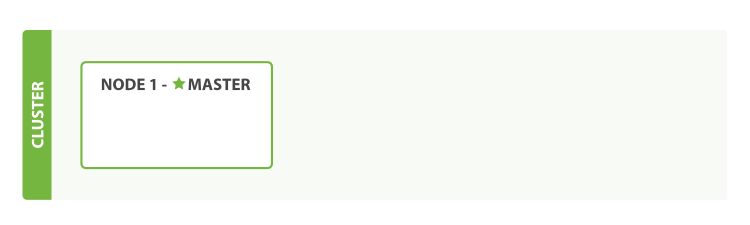
\includegraphics[width=.8\textwidth]{img/empty_cluster.png}
\caption{An empty cluster.}
\label{fig:empty-cluster}
\end{figure}

We would like to remind the problem of large amount of the data in an index mentioned in \autoref{index}. ElasticSearch solves this by splitting the index into the user-defined amount of \emph{shards}. \emph{Shard} is an independent and fully-functional index, capable of searching and indexing by its own.
The usage of shards is fully transparent to the user. In addition, ElasticSearch provides a possibility of creating copies of the shards, called \emph{replicas}. \emph{Replicas} are 1:1 clones of shards, used to ensure high availability of the indexed data. If new data is inserted into the primary shard, it is copied to its replica as well.
The replicas are also used to speed up the search by working concurrently with the shards.
An example of simple commonly used cluster is shown in \autoref{fig:replicas} that contains three shards and one replica for each shard.
\begin{figure}
\centering
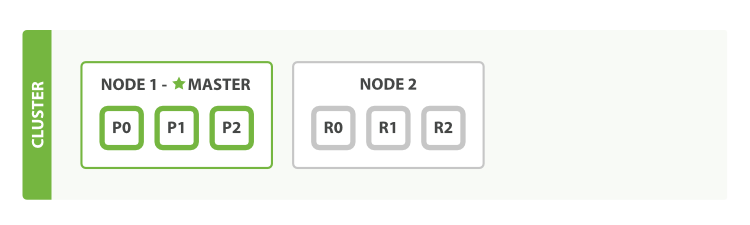
\includegraphics[width=.8\textwidth]{img/replicas.png}
\caption{A cluster with one node Master that is subdivided into three shards P0, P1 and P2. In the node 2, there is one replica shard (R0, R1, R2) for each primary shard.}
\label{fig:replicas}
\end{figure}

\subsubsection{Result score}
ElasticSearch uses \emph{Lucene's practical scoring function}~\cite{elastic} for ranking the matches.
The formula is as follows:
\begin{align*}
\centering
\textrm{s}(q,d) = \textrm{nq}(q) \cdot \textrm{c}(q,d) \cdot \sum_{t \in q}\textrm{f}(t,d) \cdot \textrm{if}(t)^2 \cdot\textrm{b}(t) \cdot \textrm{nt}(t,d),
\end{align*}
where
\begin{itemize}
\item $s(q,d)$ is the final relevance score of the query $q$ in the document $d$,
\item $\textrm{nq}(q)$ is the query normalization factor, it is used for normalizing the query $q$ in order to be able to compare it to the others,
\item $\textrm{c}(q,d)$ is the coordination factor, used to add additional score to the documents that contain higher percentage of the query terms,
\item $\textrm{f}(t,d)$ is the frequency of the term $t$ in the document $d$,
\item $\textrm{if}(t)$ is the frequency of the term $t$ in the inverted index,
\item $\textrm{b}(t)$ is a boost to the term $t$ for the query $q$, and
\item $\textrm{nt}(t,d)$ is the field-length normalization. The shorter the field, the higher the weight.
\end{itemize}

We believe that ElasticSearch is a great choice for performing the full-text search in the database of indexed e-mails as it is provides strong performance and simple interface.

\section{Application to mail indexing}
Short response time for searching in e-mails is necessary for modern e-mail user interface. 
To provide this feature, we parse the information from an e-mail message and index it into the respective fields of ElasticSearch's index. The analyzed fields are \texttt{subject}, \texttt{text}, \texttt{to} and \texttt{from}. Non-analyzed fields are \texttt{messageid}, \texttt{references} and \texttt{tag} as we want an exact match and not similarity match. The last used field is \texttt{date} which is not only analyzed but also mapped (by standard date formats) because we want the results to be sorted primarily by the date and then ranked by the relevance.

Not only user-defined searches but also many other functions are handled by ElasticSearch. Grouping of the emails by references is done by ElasticSearch. As the e-mail directory-based hierarchy is replaced by tags, these are searched by ElasticSearch as well.
